\section{APX-completeness for segments parallel to axis}
\label{section:segment_apx}

\subsection{Definition of  MAX-(3,3)-SAT problem}
Here we define MAXSAT problem.

\begin{tw}{
	\label{hastadtheorem}
	\textbf{\cite{hastad}}
	Assume NP $\not\subseteq$ $DTIME(2^{O(\log n \log \log n)})$.
	Then, there exists such constant $c > 0$, such for
	$$\epsilon' = \frac{c \log \log \log n}{\log \log n}$$ 
	satifiable 3-SAT formulas cannot be distinguished from
	3-SAT formulas where only $7/8+\epsilon'$ of~the clauses
	can be satisfied in polynomial time.
}\end{tw}

\begin{tw}{
	\label{apxconstruction}
	Given an instance of  MAX-(3,3)-SAT 
	with $n$ variables and optimal result $k$,
	we can construct an instance of axis-parallel segments in 2D,
	which optimal result (even with 1/2-extension) is exactly $17n - k$.
}\end{tw}

\begin{tw}{
	\textbf{(axis-parallel segment set cover with 1/2-extension is APX-hard)}.	
	For every $\epsilon > 0$,
	there doesn't exist an $(1-\epsilon)$-approximation scheme
	for unweighted geometric set cover
	with axis-parallel segments in 2D (even with 1/2-extension)
	(problem is APX-hard).
}\end{tw}

\paragraph{Proof.}
Take any $\epsilon > 0$.
Take such $n$, that $\epsilon'$ from \ref{hastadtheorem}
is not greater than $max(\epsilon, 1/2)$.

Let's assume that there exists an $(1-\epsilon)$-approximation scheme
for unweighted geometric set cover with axis-pararell segments in 2D.
We will construct an algorithm distinguishing instances of MAX-(3,3)-SAT
in \ref{hastadtheorem}.
Take two instances to be distinguished and using \ref{apxconstruction}
let's construct two instances of geometric set cover,
name the one constructed from satisfiable 3-SAT $I_1$
and the unsatisfiable 3-SAT as $I_0$.

Use $(1-\epsilon)$-approximation scheme for instances of geometric
set cover, let's name the result of this approximation
for an instance of problem $I$ as $approx(I)$.

$$approx(I_1) \ge (1-\epsilon)17n > 16\frac{1}{8}n - \epsilon' \ge approx(I_2)$$ 

So we can distinguish these instances, since the satifiable instance
will always yield greater result in approximation scheme.

Therefore such approximation scheme cannot exist.

\subsection{Reduction construction}

Let's take some instance of  MAX-(3,3)-SAT with
variables $x_1, x_2 \ldots x_n$
and clauses $C_1, C_2 \dots C_n$.

We will create gadgets for choosing the value
of variables (\textit{true} or \textit{false}) and checking
if the clauses are met (any of the variables were chosen).

\begin{figure}[h]
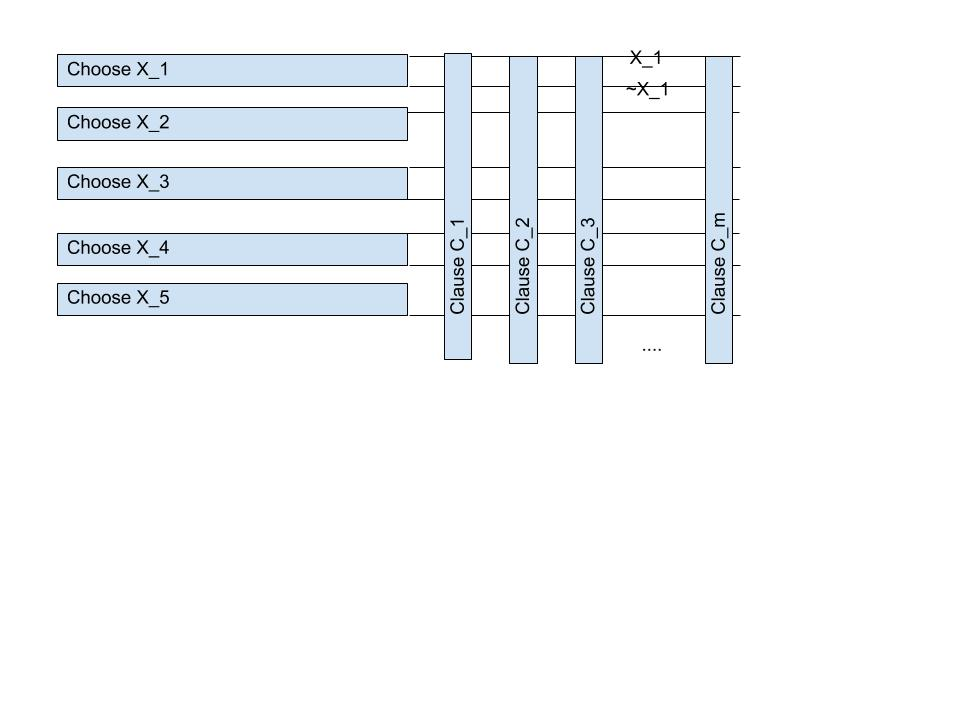
\includegraphics[width=0.7\textwidth]{segment_apx_sketch.jpg}
\caption{General scheme of reduction.}
\label{fig:segment_apx}
\end{figure}

\subsubsection{Choose $x_i$ gadget}
\begin{figure}[h]
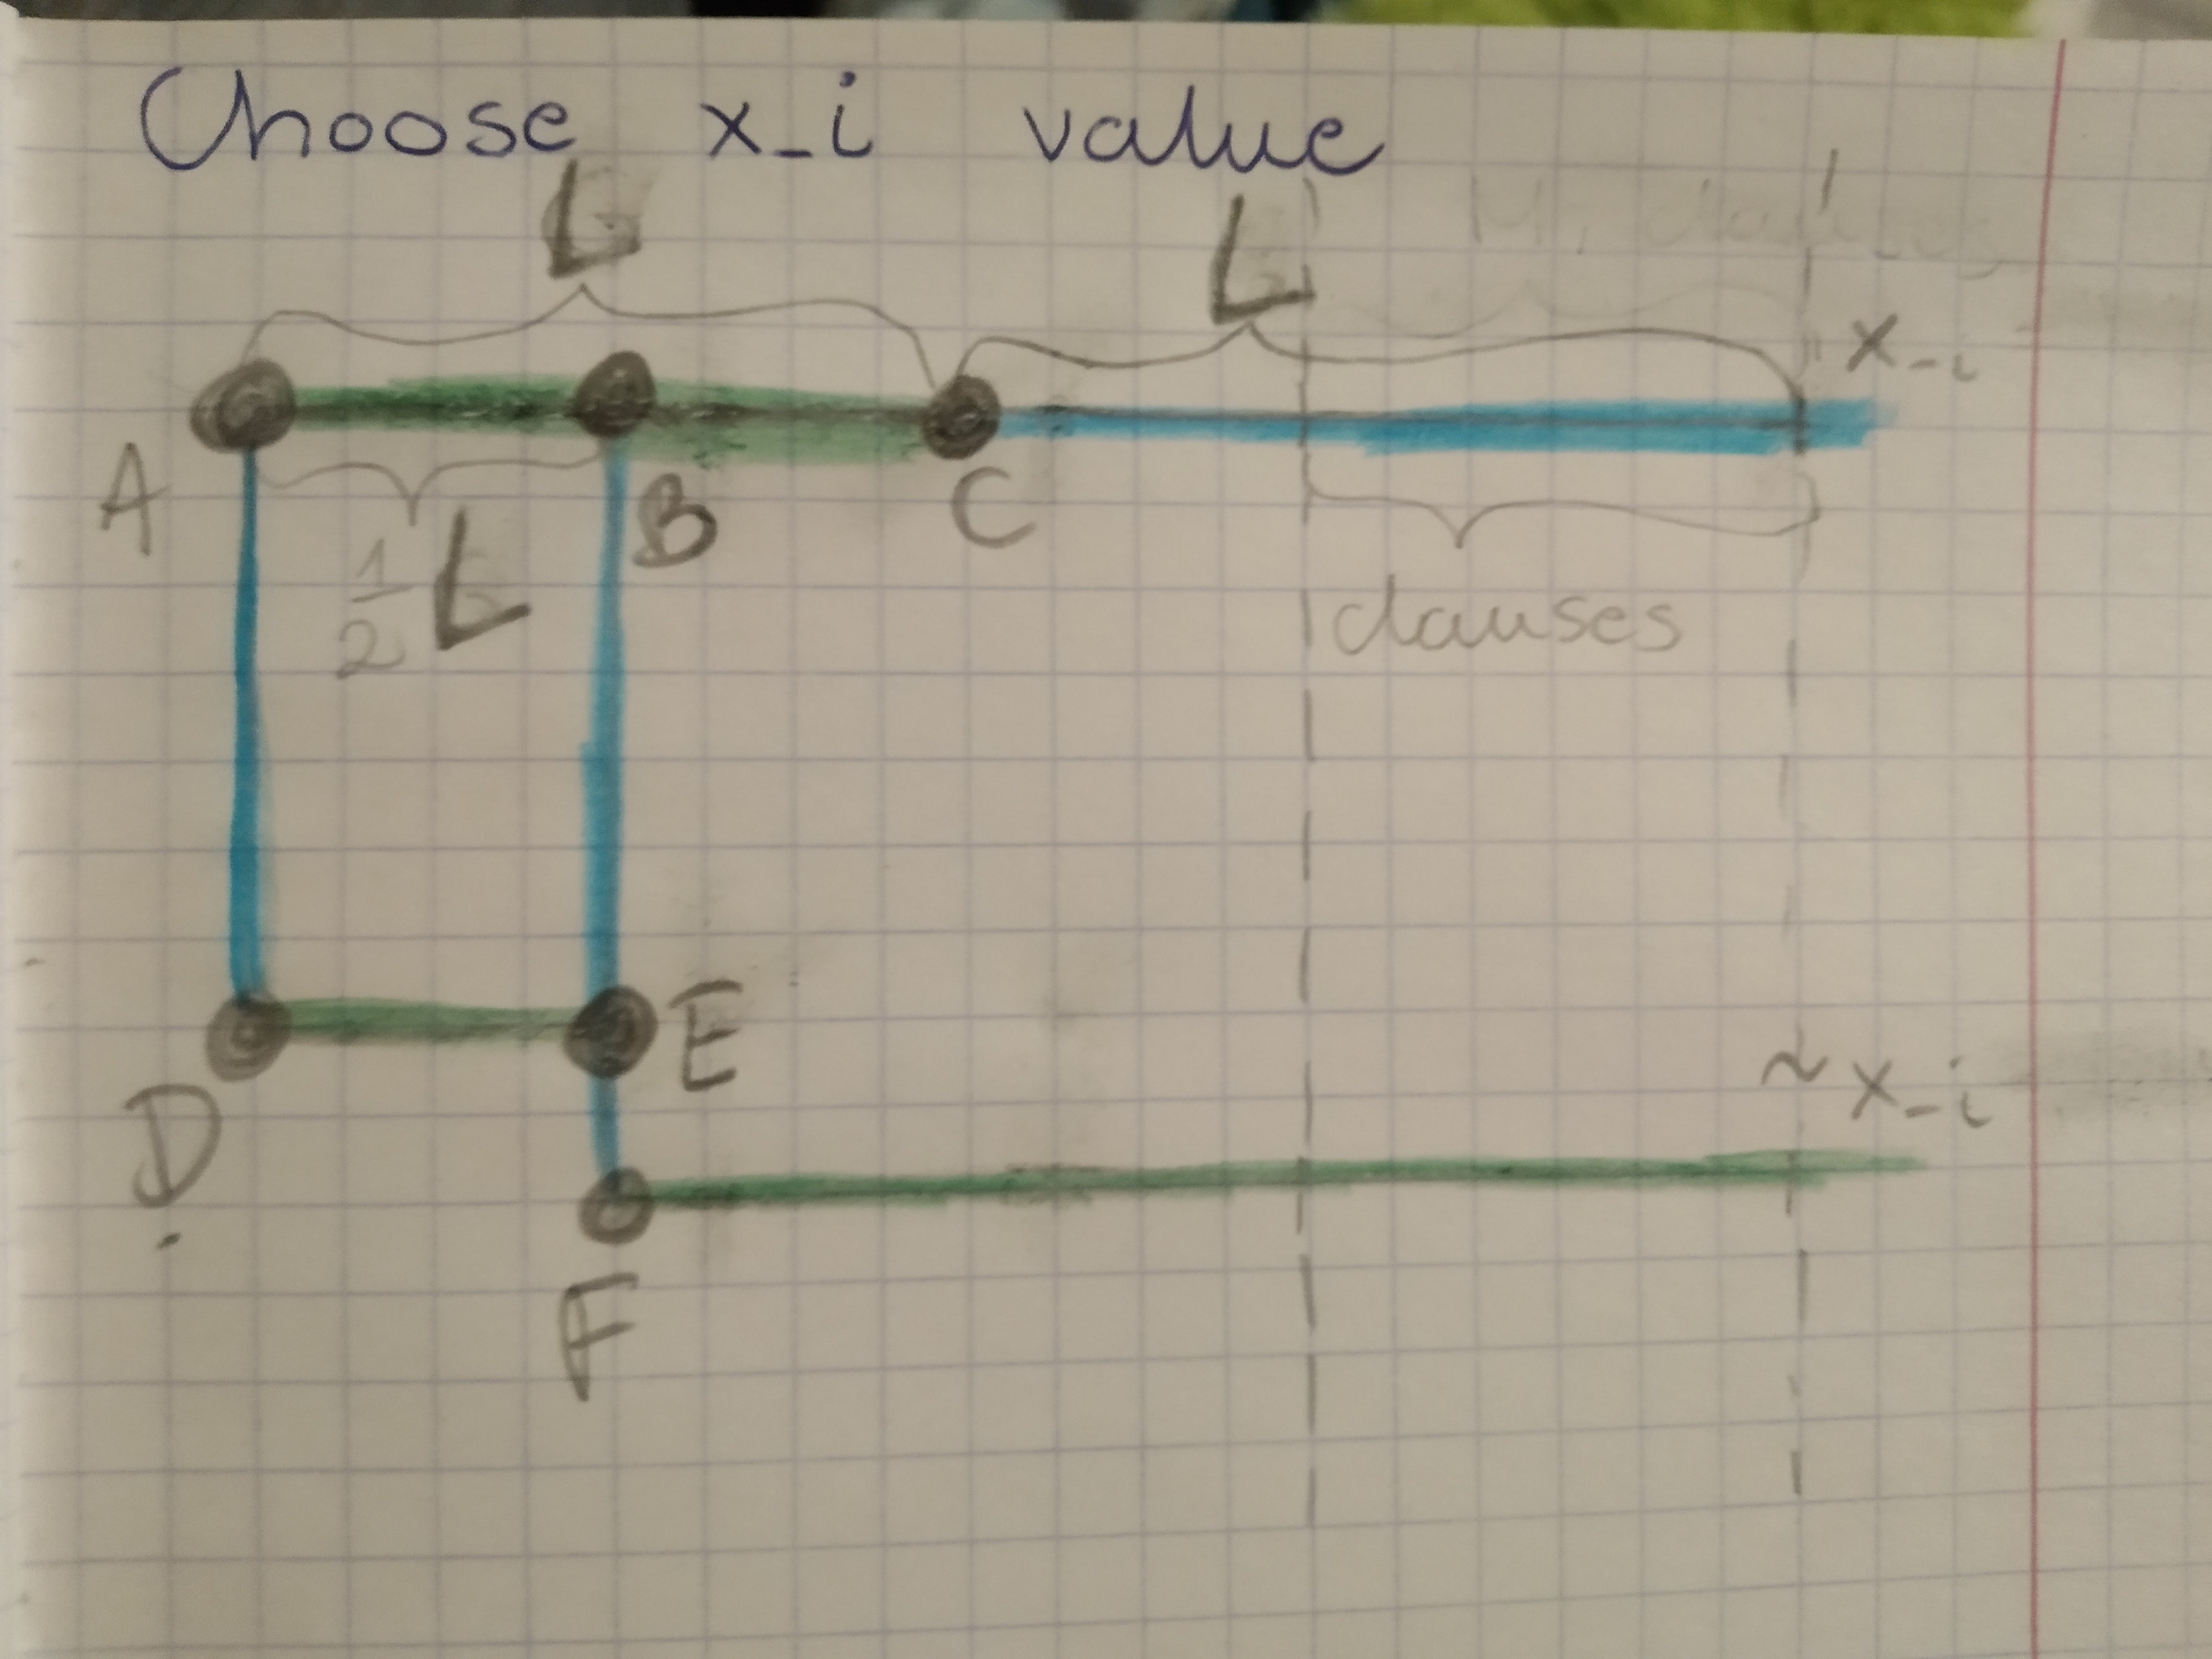
\includegraphics[width=0.6\textwidth]{choose_x_gadget.jpg}
\caption{Scheme of choose $x_i$ gadget.}
\label{fig:choose_x_gadget}
\end{figure}
In Figure~\ref{fig:choose_x_gadget},
we show a gadget that simulates a single variable $x_i$.
It consists of six points A, B, C, D, E, F, and several segments.
Selecting the segment marked with $x_i$
to the solution will correspond to setting $x_i$ to \textit{true},
while selecting the segment marked with $\neg x_i$
to setting $x_i$ to \textit{false}.
In the following lemmas,
we show that this construction indeed models a binary variable.

First, note that in the gadget
there are exactly two sets of three segments
that cover all points $A, B, C, D, E, F$.
These two sets of segments are marked in
Figure~\ref{fig:choose_x_gadget} in blue and green, respectively.

\begin{lemma}
Points $A, B, C, D, E, F$ cannot be covered using less than
3 segments (even with $1/2$-extensions).
\end{lemma}
\paragraph{Proof.}
We need to take at least one segment on line $ABC$,
because it's the only way to cover $C$.
All other points ($D, E, F$) are not colinear,
so we need at least 2 other segments to cover them.

\begin{lemma}
If we choose both segments $x_i$ and $\neg x_i$, we need to use at
least 4 segments to cover all points $A, B, C, D, E, F$
(even with $1/2$-extensions).
\end{lemma}

\paragraph{Proof.}
Choosing both segments $x_i$ and $\neg x_i$
we only cover points $C$
(becuase $B$ is too far away to be covered with $1/2$-extension)
and $F$.

The remaining points ($A, B, D, E$) are not colinear,
so we need at least two more segments to cover them.

\paragraph{Robustness to $1/2$-extension.}
Take a look at Figure~\ref{fig:segment_apx}.
The points will be included in choose gadgets (horizontal boxes)
and clause gadgets (vertical boxes).

Since segment $AC$ is very long
and colinear with $x_i$, after $1/2$-extension
it will cover a significant part of segment $x_i$,
even though $x_i$ will not be chosen.

If we put all the clause gadgets in the area
marked with \textbf{clauses} at gadget scheme in Figure~\ref{fig:choose_x_gadget},
it is enough to prove that $AC$ will not cover any points
in the \textbf{clauses} area even with $1/2$-extensions.

\begin{lemma}
No points in \textbf{clauses} area can be covered
by $AC$ with $1/2$-extension.
\end{lemma}

\paragraph{Proof.}
Bear in mind that length of $AC$ is equal to length of $x_i$.
Area \textbf{clauses} takes a second half
of the segment $x_i$ and $AC$ after extension will cover the first
half of segment $x_i$.

\subsubsection{Clause gadget}
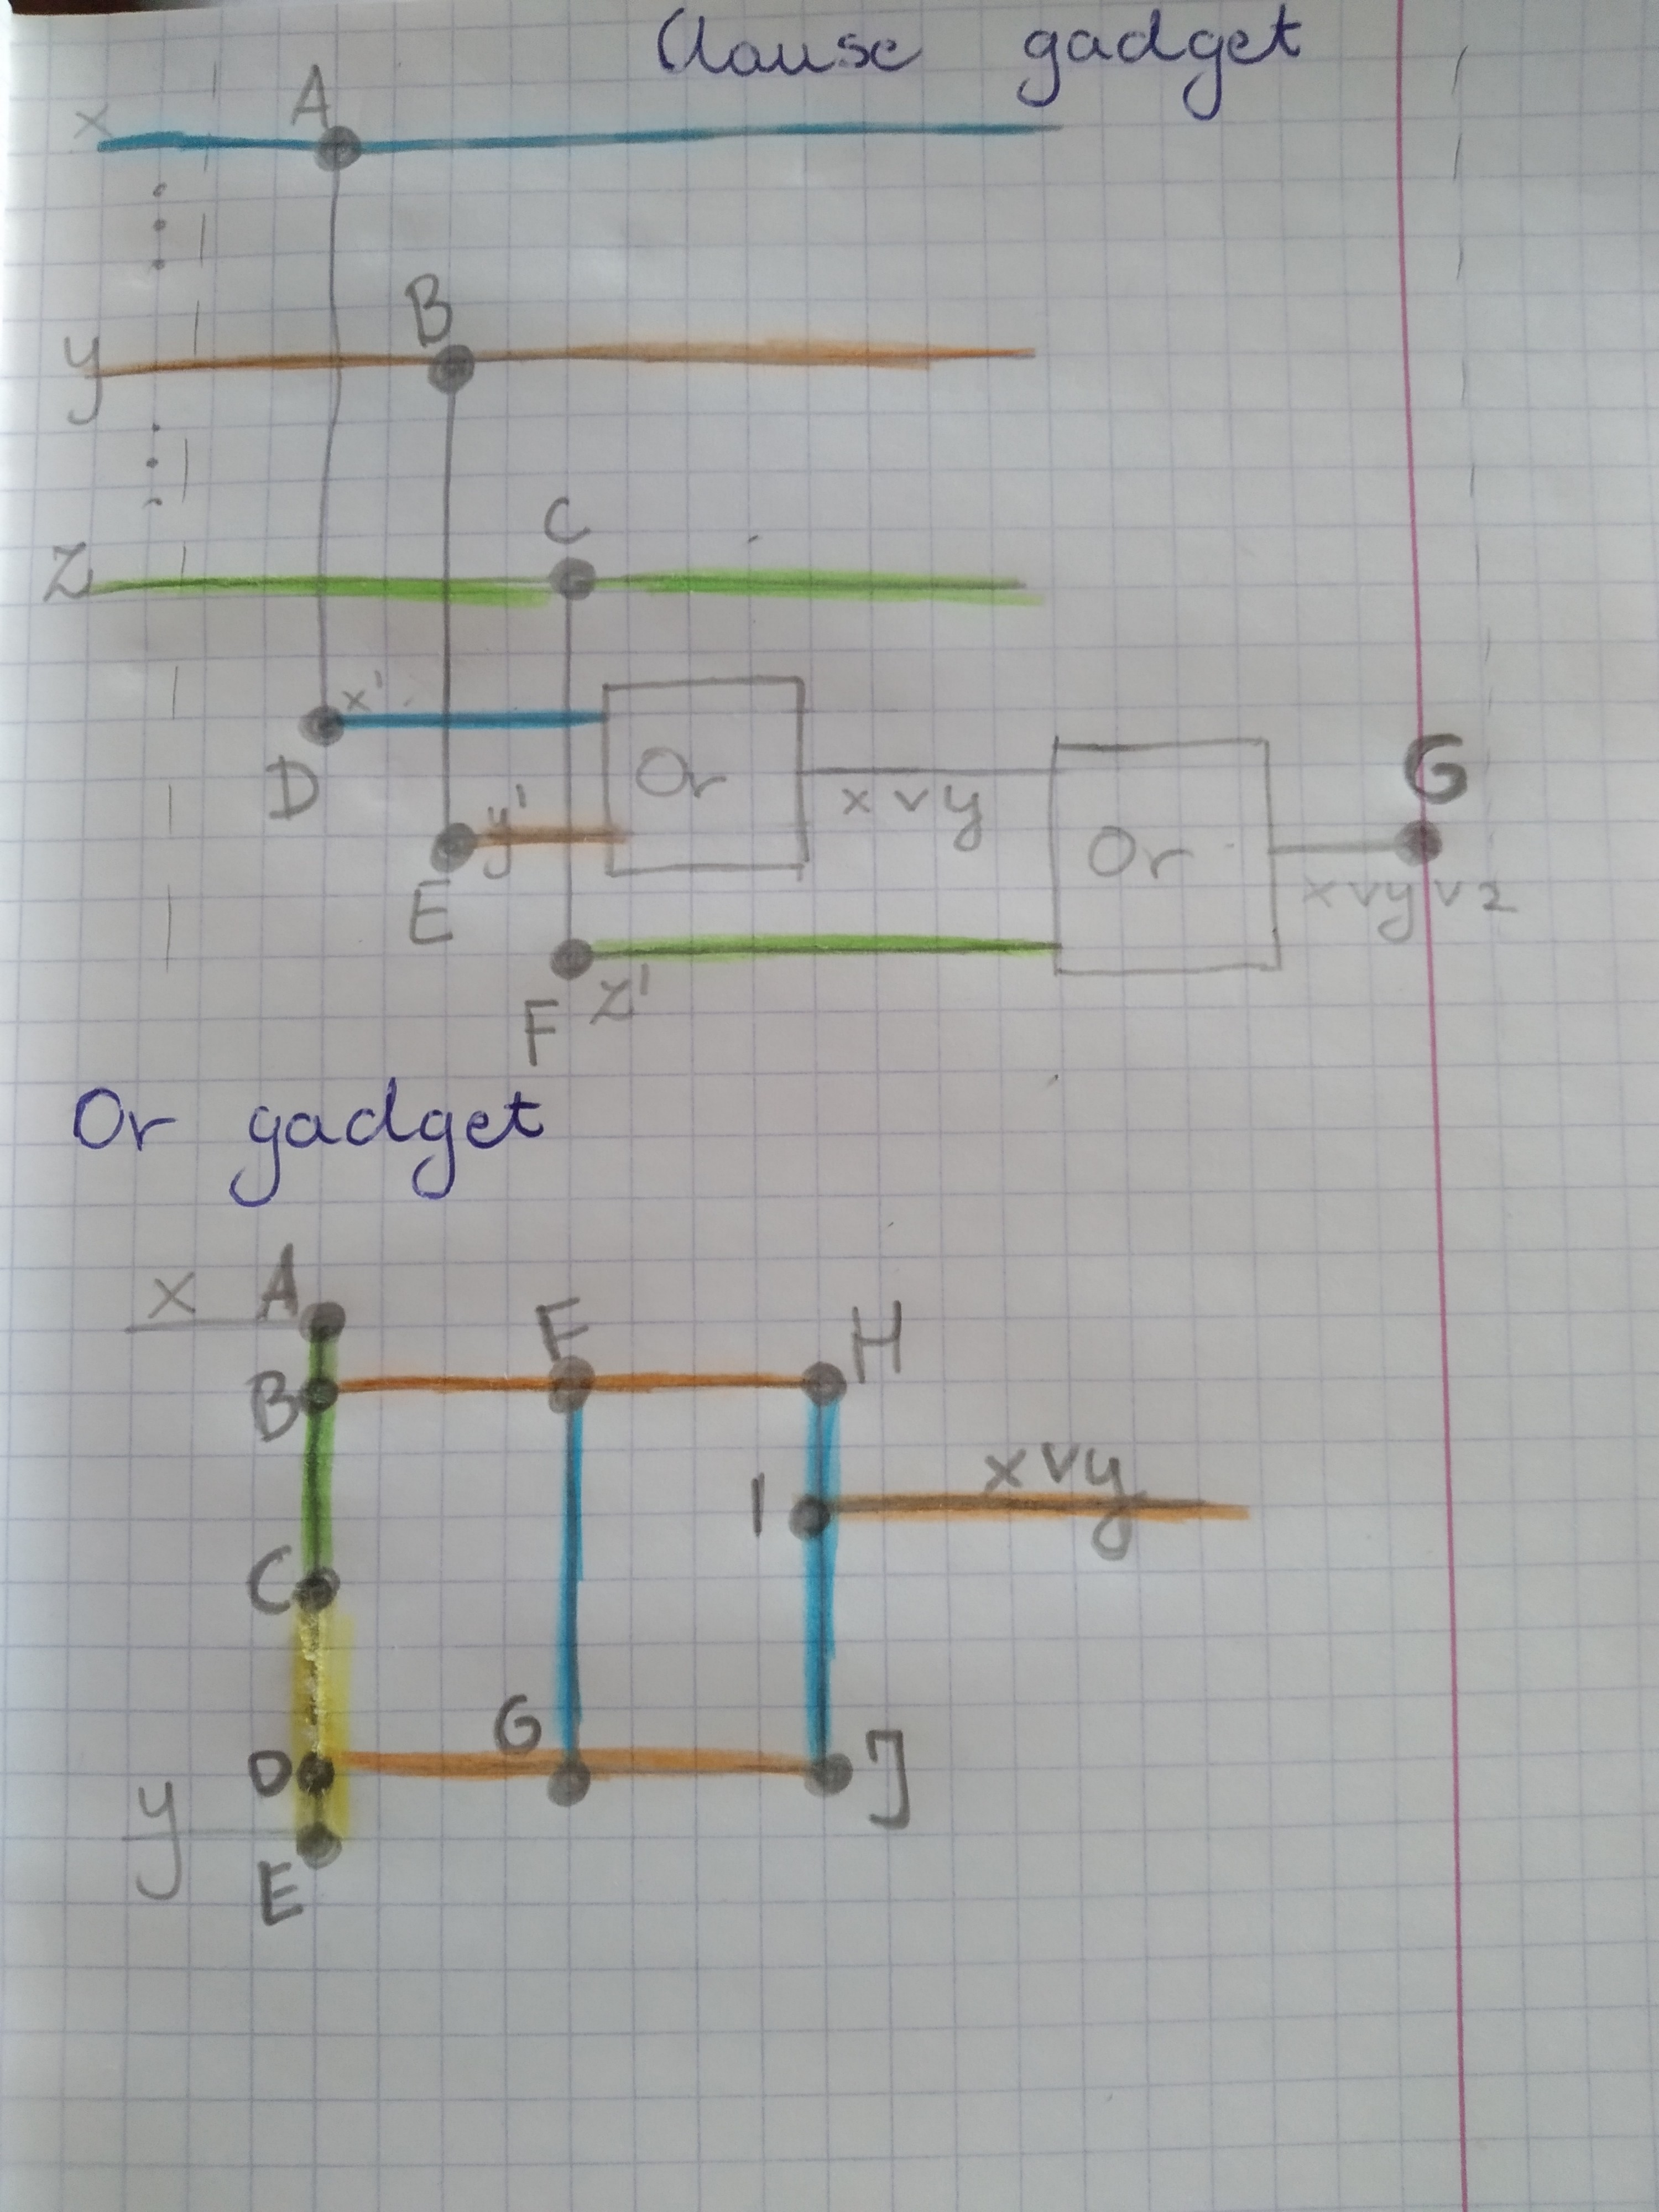
\includegraphics[width=0.6\textwidth]{clause_gadget.jpg}

\begin{lemma}
In order to cover $D$ ($E, F$) point at least one
of the segments $AD$ ($BE, CF$) or $x'$ ($y', z'$).
\end{lemma}

\begin{lemma}
Points $A$ and $D$ can be covered
with one additional segment $x'$
only if $x$ is already chosen.
Otherwise they can be covered with one segment
only by using $AD$.
\end{lemma}

\begin{lemma}
Points $A, B, C, D, E, F, G$ can be covered with 
3 or 4 segments, depending if at least one of the segments
$x, y, z$ was previously chosen.
\end{lemma}

\subsubsection{Or gadget}
\begin{lemma}
Points $A, B, C, D, E, F, G, H, I, J$ can be covered using
at least 4 segments even with $1/2$-extension.
\end{lemma}

\begin{lemma}
Points $A, B, C, D, E, F, G, H, I, J$ can be covered using
4 segments and segment $x \lor y$ can be chosen
even with $1/2$-extension
only if at least one of the segments $x$ or $y$ is chosen.
\end{lemma}

\subsection{Proof that construction is sound}
\begin{lemma}
If there exists setting of values of variables that exactly $k$
clauses are satisfied, we can cover all the points
with $3n + 11m + (m-k)$ segments.
\end{lemma}

\begin{lemma}
If there exists cover with $k$ segments,
then also there exists solution for MAX-(3,3)-SAT.

TODO: Formulate this lemma better.
\end{lemma}
